\documentclass[1p]{elsarticle_modified}
%\bibliographystyle{elsarticle-num}

%\usepackage[colorlinks]{hyperref}
%\usepackage{abbrmath_seonhwa} %\Abb, \Ascr, \Acal ,\Abf, \Afrak
\usepackage{amsfonts}
\usepackage{amssymb}
\usepackage{amsmath}
\usepackage{amsthm}
\usepackage{scalefnt}
\usepackage{amsbsy}
\usepackage{kotex}
\usepackage{caption}
\usepackage{subfig}
\usepackage{color}
\usepackage{graphicx}
\usepackage{xcolor} %% white, black, red, green, blue, cyan, magenta, yellow
\usepackage{float}
\usepackage{setspace}
\usepackage{hyperref}

\usepackage{tikz}
\usetikzlibrary{arrows}

\usepackage{multirow}
\usepackage{array} % fixed length table
\usepackage{hhline}

%%%%%%%%%%%%%%%%%%%%%
\makeatletter
\renewcommand*\env@matrix[1][\arraystretch]{%
	\edef\arraystretch{#1}%
	\hskip -\arraycolsep
	\let\@ifnextchar\new@ifnextchar
	\array{*\c@MaxMatrixCols c}}
\makeatother %https://tex.stackexchange.com/questions/14071/how-can-i-increase-the-line-spacing-in-a-matrix
%%%%%%%%%%%%%%%

\usepackage[normalem]{ulem}

\newcommand{\msout}[1]{\ifmmode\text{\sout{\ensuremath{#1}}}\else\sout{#1}\fi}
%SOURCE: \msout is \stkout macro in https://tex.stackexchange.com/questions/20609/strikeout-in-math-mode

\newcommand{\cancel}[1]{
	\ifmmode
	{\color{red}\msout{#1}}
	\else
	{\color{red}\sout{#1}}
	\fi
}

\newcommand{\add}[1]{
	{\color{blue}\uwave{#1}}
}

\newcommand{\replace}[2]{
	\ifmmode
	{\color{red}\msout{#1}}{\color{blue}\uwave{#2}}
	\else
	{\color{red}\sout{#1}}{\color{blue}\uwave{#2}}
	\fi
}

\newcommand{\Sol}{\mathcal{S}} %segment
\newcommand{\D}{D} %diagram
\newcommand{\A}{\mathcal{A}} %arc


%%%%%%%%%%%%%%%%%%%%%%%%%%%%%5 test

\def\sl{\operatorname{\textup{SL}}(2,\Cbb)}
\def\psl{\operatorname{\textup{PSL}}(2,\Cbb)}
\def\quan{\mkern 1mu \triangleright \mkern 1mu}

\theoremstyle{definition}
\newtheorem{thm}{Theorem}[section]
\newtheorem{prop}[thm]{Proposition}
\newtheorem{lem}[thm]{Lemma}
\newtheorem{ques}[thm]{Question}
\newtheorem{cor}[thm]{Corollary}
\newtheorem{defn}[thm]{Definition}
\newtheorem{exam}[thm]{Example}
\newtheorem{rmk}[thm]{Remark}
\newtheorem{alg}[thm]{Algorithm}

\newcommand{\I}{\sqrt{-1}}
\begin{document}

%\begin{frontmatter}
%
%\title{Boundary parabolic representations of knots up to 8 crossings}
%
%%% Group authors per affiliation:
%\author{Yunhi Cho} 
%\address{Department of Mathematics, University of Seoul, Seoul, Korea}
%\ead{yhcho@uos.ac.kr}
%
%
%\author{Seonhwa Kim} %\fnref{s_kim}}
%\address{Center for Geometry and Physics, Institute for Basic Science, Pohang, 37673, Korea}
%\ead{ryeona17@ibs.re.kr}
%
%\author{Hyuk Kim}
%\address{Department of Mathematical Sciences, Seoul National University, Seoul 08826, Korea}
%\ead{hyukkim@snu.ac.kr}
%
%\author{Seokbeom Yoon}
%\address{Department of Mathematical Sciences, Seoul National University, Seoul, 08826,  Korea}
%\ead{sbyoon15@snu.ac.kr}
%
%\begin{abstract}
%We find all boundary parabolic representation of knots up to 8 crossings.
%
%\end{abstract}
%\begin{keyword}
%    \MSC[2010] 57M25 
%\end{keyword}
%
%\end{frontmatter}

%\linenumbers
%\tableofcontents
%
\newcommand\colored[1]{\textcolor{white}{\rule[-0.35ex]{0.8em}{1.4ex}}\kern-0.8em\color{red} #1}%
%\newcommand\colored[1]{\textcolor{white}{ #1}\kern-2.17ex	\textcolor{white}{ #1}\kern-1.81ex	\textcolor{white}{ #1}\kern-2.15ex\color{red}#1	}

{\Large $\underline{11a_{323}~(K11a_{323})}$}

\setlength{\tabcolsep}{10pt}
\renewcommand{\arraystretch}{1.6}
\vspace{1cm}\begin{tabular}{m{100pt}>{\centering\arraybackslash}m{274pt}}
\multirow{5}{120pt}{
	\centering
	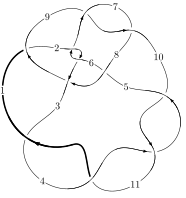
\includegraphics[width=112pt]{../../../GIT/diagram.site/Diagrams/png/572_11a_323.png}\\
\ \ \ A knot diagram\footnotemark}&
\allowdisplaybreaks
\textbf{Linearized knot diagam} \\
\cline{2-2}
 &
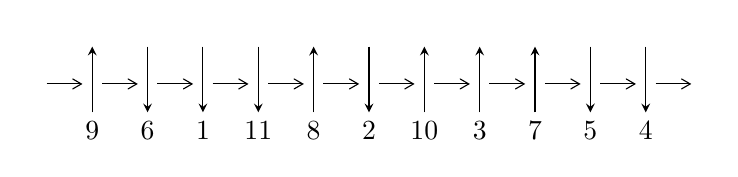
\begin{tikzpicture}[x=20pt, y=17pt]
	% nodes
	\node (C0) at (0, 0) {};
	\node (C1) at (1, 0) {};
	\node (C1U) at (1, +1) {};
	\node (C1D) at (1, -1) {9};

	\node (C2) at (2, 0) {};
	\node (C2U) at (2, +1) {};
	\node (C2D) at (2, -1) {6};

	\node (C3) at (3, 0) {};
	\node (C3U) at (3, +1) {};
	\node (C3D) at (3, -1) {1};

	\node (C4) at (4, 0) {};
	\node (C4U) at (4, +1) {};
	\node (C4D) at (4, -1) {11};

	\node (C5) at (5, 0) {};
	\node (C5U) at (5, +1) {};
	\node (C5D) at (5, -1) {8};

	\node (C6) at (6, 0) {};
	\node (C6U) at (6, +1) {};
	\node (C6D) at (6, -1) {2};

	\node (C7) at (7, 0) {};
	\node (C7U) at (7, +1) {};
	\node (C7D) at (7, -1) {10};

	\node (C8) at (8, 0) {};
	\node (C8U) at (8, +1) {};
	\node (C8D) at (8, -1) {3};

	\node (C9) at (9, 0) {};
	\node (C9U) at (9, +1) {};
	\node (C9D) at (9, -1) {7};

	\node (C10) at (10, 0) {};
	\node (C10U) at (10, +1) {};
	\node (C10D) at (10, -1) {5};

	\node (C11) at (11, 0) {};
	\node (C11U) at (11, +1) {};
	\node (C11D) at (11, -1) {4};
	\node (C12) at (12, 0) {};

	% arrows
	\draw[->,>={angle 60}]
	(C0) edge (C1) (C1) edge (C2) (C2) edge (C3) (C3) edge (C4) (C4) edge (C5) (C5) edge (C6) (C6) edge (C7) (C7) edge (C8) (C8) edge (C9) (C9) edge (C10) (C10) edge (C11) (C11) edge (C12) ;	\draw[->,>=stealth]
	(C1D) edge (C1U) (C2U) edge (C2D) (C3U) edge (C3D) (C4U) edge (C4D) (C5D) edge (C5U) (C6U) edge (C6D) (C7D) edge (C7U) (C8D) edge (C8U) (C9D) edge (C9U) (C10U) edge (C10D) (C11U) edge (C11D) ;
	\end{tikzpicture} \\
\hhline{~~} \\& 
\textbf{Solving Sequence} \\ \cline{2-2} 
 &
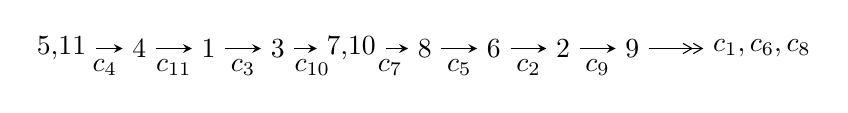
\begin{tikzpicture}[x=25pt, y=7pt]
	% node
	\node (A0) at (-1/8, 0) {5,11};
	\node (A1) at (1, 0) {4};
	\node (A2) at (2, 0) {1};
	\node (A3) at (3, 0) {3};
	\node (A4) at (65/16, 0) {7,10};
	\node (A5) at (41/8, 0) {8};
	\node (A6) at (49/8, 0) {6};
	\node (A7) at (57/8, 0) {2};
	\node (A8) at (65/8, 0) {9};
	\node (C1) at (1/2, -1) {$c_{4}$};
	\node (C2) at (3/2, -1) {$c_{11}$};
	\node (C3) at (5/2, -1) {$c_{3}$};
	\node (C4) at (7/2, -1) {$c_{10}$};
	\node (C5) at (37/8, -1) {$c_{7}$};
	\node (C6) at (45/8, -1) {$c_{5}$};
	\node (C7) at (53/8, -1) {$c_{2}$};
	\node (C8) at (61/8, -1) {$c_{9}$};
	\node (A9) at (10, 0) {$c_{1},c_{6},c_{8}$};

	% edge
	\draw[->,>=stealth]	
	(A0) edge (A1) (A1) edge (A2) (A2) edge (A3) (A3) edge (A4) (A4) edge (A5) (A5) edge (A6) (A6) edge (A7) (A7) edge (A8) ;
	\draw[->>,>={angle 60}]	
	(A8) edge (A9);
\end{tikzpicture} \\ 

\end{tabular} \\

\footnotetext{
The image of knot diagram is generated by the software ``\textbf{Draw programme}" developed by Andrew Bartholomew(\url{http://www.layer8.co.uk/maths/draw/index.htm\#Running-draw}), where we modified some parts for our purpose(\url{https://github.com/CATsTAILs/LinksPainter}).
}\phantom \\ \newline 
\centering \textbf{Ideals for irreducible components\footnotemark of $X_{\text{par}}$} 
 
\begin{align*}
I^u_{1}&=\langle 
2.31401\times10^{21} u^{43}-3.54437\times10^{21} u^{42}+\cdots+8.57234\times10^{19} b+4.94843\times10^{21},\\
\phantom{I^u_{1}}&\phantom{= \langle  }-5.89751\times10^{21} u^{43}+9.06194\times10^{21} u^{42}+\cdots+8.57234\times10^{19} a-1.26997\times10^{22},\;u^{44}-2 u^{43}+\cdots+5 u-1\rangle \\
I^u_{2}&=\langle 
u^2+5 b+7 u+4,\;-4 u^2+5 a+2 u-6,\;u^3+u^2+2 u+1\rangle \\
\\
\end{align*}
\raggedright * 2 irreducible components of $\dim_{\mathbb{C}}=0$, with total 47 representations.\\
\footnotetext{All coefficients of polynomials are rational numbers. But the coefficients are sometimes approximated in decimal forms when there is not enough margin.}
\newpage
\renewcommand{\arraystretch}{1}
\centering \section*{I. $I^u_{1}= \langle 2.31\times10^{21} u^{43}-3.54\times10^{21} u^{42}+\cdots+8.57\times10^{19} b+4.95\times10^{21},\;-5.90\times10^{21} u^{43}+9.06\times10^{21} u^{42}+\cdots+8.57\times10^{19} a-1.27\times10^{22},\;u^{44}-2 u^{43}+\cdots+5 u-1 \rangle$}
\flushleft \textbf{(i) Arc colorings}\\
\begin{tabular}{m{7pt} m{180pt} m{7pt} m{180pt} }
\flushright $a_{5}=$&$\begin{pmatrix}1\\0\end{pmatrix}$ \\
\flushright $a_{11}=$&$\begin{pmatrix}0\\u\end{pmatrix}$ \\
\flushright $a_{4}=$&$\begin{pmatrix}1\\- u^2\end{pmatrix}$ \\
\flushright $a_{1}=$&$\begin{pmatrix}- u\\u^3+u\end{pmatrix}$ \\
\flushright $a_{3}=$&$\begin{pmatrix}u^2+1\\- u^4-2 u^2\end{pmatrix}$ \\
\flushright $a_{7}=$&$\begin{pmatrix}68.7969 u^{43}-105.711 u^{42}+\cdots-427.419 u+148.148\\-26.9939 u^{43}+41.3466 u^{42}+\cdots+164.286 u-57.7256\end{pmatrix}$ \\
\flushright $a_{10}=$&$\begin{pmatrix}u\\u\end{pmatrix}$ \\
\flushright $a_{8}=$&$\begin{pmatrix}48.3780 u^{43}-74.2119 u^{42}+\cdots-300.591 u+103.624\\-47.4129 u^{43}+72.8461 u^{42}+\cdots+291.114 u-102.249\end{pmatrix}$ \\
\flushright $a_{6}=$&$\begin{pmatrix}-21.2354 u^{43}+32.3030 u^{42}+\cdots+140.637 u-45.5104\\64.6016 u^{43}-99.5702 u^{42}+\cdots-387.835 u+137.751\end{pmatrix}$ \\
\flushright $a_{2}=$&$\begin{pmatrix}-6.60822 u^{43}+11.0300 u^{42}+\cdots+33.2318 u-11.2429\\-30.3756 u^{43}+47.4335 u^{42}+\cdots+187.153 u-65.4032\end{pmatrix}$ \\
\flushright $a_{9}=$&$\begin{pmatrix}7.06760 u^{43}-10.5739 u^{42}+\cdots-44.3693 u+13.4967\\-31.4705 u^{43}+48.2831 u^{42}+\cdots+193.366 u-67.6179\end{pmatrix}$\\ \flushright $a_{9}=$&$\begin{pmatrix}7.06760 u^{43}-10.5739 u^{42}+\cdots-44.3693 u+13.4967\\-31.4705 u^{43}+48.2831 u^{42}+\cdots+193.366 u-67.6179\end{pmatrix}$\\&\end{tabular}
\flushleft \textbf{(ii) Obstruction class $= -1$}\\~\\
\flushleft \textbf{(iii) Cusp Shapes $= \frac{98838962520190550252816}{428617191062252656975} u^{43}-\frac{152658479968934161876903}{428617191062252656975} u^{42}+\cdots-\frac{605374312863961326763079}{428617191062252656975} u+\frac{218640669764653807216074}{428617191062252656975}$}\\~\\
\newpage\renewcommand{\arraystretch}{1}
\flushleft \textbf{(iv) u-Polynomials at the component}\newline \\
\begin{tabular}{m{50pt}|m{274pt}}
Crossings & \hspace{64pt}u-Polynomials at each crossing \\
\hline $$\begin{aligned}c_{1}\end{aligned}$$&$\begin{aligned}
&5(5 u^{44}-21 u^{43}+\cdots+864 u+823)
\end{aligned}$\\
\hline $$\begin{aligned}c_{2},c_{6}\end{aligned}$$&$\begin{aligned}
&u^{44}+2 u^{43}+\cdots+u-1
\end{aligned}$\\
\hline $$\begin{aligned}c_{3},c_{4},c_{10}\\c_{11}\end{aligned}$$&$\begin{aligned}
&u^{44}-2 u^{43}+\cdots+5 u-1
\end{aligned}$\\
\hline $$\begin{aligned}c_{5}\end{aligned}$$&$\begin{aligned}
&5(5 u^{44}-2 u^{43}+\cdots+23513 u+5383)
\end{aligned}$\\
\hline $$\begin{aligned}c_{7},c_{9}\end{aligned}$$&$\begin{aligned}
&u^{44}+4 u^{43}+\cdots+16 u-25
\end{aligned}$\\
\hline $$\begin{aligned}c_{8}\end{aligned}$$&$\begin{aligned}
&u^{44}+u^{43}+\cdots-220 u+200
\end{aligned}$\\
\hline
\end{tabular}\\~\\
\newpage\renewcommand{\arraystretch}{1}
\flushleft \textbf{(v) Riley Polynomials at the component}\newline \\
\begin{tabular}{m{50pt}|m{274pt}}
Crossings & \hspace{64pt}Riley Polynomials at each crossing \\
\hline $$\begin{aligned}c_{1}\end{aligned}$$&$\begin{aligned}
&25(25 y^{44}-671 y^{43}+\cdots-2153826 y+677329)
\end{aligned}$\\
\hline $$\begin{aligned}c_{2},c_{6}\end{aligned}$$&$\begin{aligned}
&y^{44}+30 y^{43}+\cdots-23 y+1
\end{aligned}$\\
\hline $$\begin{aligned}c_{3},c_{4},c_{10}\\c_{11}\end{aligned}$$&$\begin{aligned}
&y^{44}+54 y^{43}+\cdots-23 y+1
\end{aligned}$\\
\hline $$\begin{aligned}c_{5}\end{aligned}$$&$\begin{aligned}
&25(25 y^{44}-914 y^{43}+\cdots-1.98283\times10^{8} y+2.89767\times10^{7})
\end{aligned}$\\
\hline $$\begin{aligned}c_{7},c_{9}\end{aligned}$$&$\begin{aligned}
&y^{44}-40 y^{43}+\cdots-9756 y+625
\end{aligned}$\\
\hline $$\begin{aligned}c_{8}\end{aligned}$$&$\begin{aligned}
&y^{44}-21 y^{43}+\cdots-482000 y+40000
\end{aligned}$\\
\hline
\end{tabular}\\~\\
\newpage\flushleft \textbf{(vi) Complex Volumes and Cusp Shapes}
$$\begin{array}{c|c|c}  
\text{Solutions to }I^u_{1}& \I (\text{vol} + \sqrt{-1}CS) & \text{Cusp shape}\\
 \hline 
\begin{aligned}
u &= \phantom{-}0.531615 + 0.932164 I \\
a &= \phantom{-}0.040863 + 0.471379 I \\
b &= -0.29401 + 1.86560 I\end{aligned}
 & \phantom{-}9.4938 - 10.7466 I & \phantom{-0.000000 } 0 \\ \hline\begin{aligned}
u &= \phantom{-}0.531615 - 0.932164 I \\
a &= \phantom{-}0.040863 - 0.471379 I \\
b &= -0.29401 - 1.86560 I\end{aligned}
 & \phantom{-}9.4938 + 10.7466 I & \phantom{-0.000000 } 0 \\ \hline\begin{aligned}
u &= \phantom{-}0.604409 + 0.897873 I \\
a &= \phantom{-}0.417373 + 0.331876 I \\
b &= -0.387595 + 1.341230 I\end{aligned}
 & \phantom{-}9.03616 + 1.64979 I & \phantom{-0.000000 } 0 \\ \hline\begin{aligned}
u &= \phantom{-}0.604409 - 0.897873 I \\
a &= \phantom{-}0.417373 - 0.331876 I \\
b &= -0.387595 - 1.341230 I\end{aligned}
 & \phantom{-}9.03616 - 1.64979 I & \phantom{-0.000000 } 0 \\ \hline\begin{aligned}
u &= -0.102848 + 0.888493 I \\
a &= -0.581285 + 0.418665 I \\
b &= -0.15348 - 1.41968 I\end{aligned}
 & \phantom{-}7.69062 + 2.11031 I & \phantom{-}11.34242 - 3.52324 I \\ \hline\begin{aligned}
u &= -0.102848 - 0.888493 I \\
a &= -0.581285 - 0.418665 I \\
b &= -0.15348 + 1.41968 I\end{aligned}
 & \phantom{-}7.69062 - 2.11031 I & \phantom{-}11.34242 + 3.52324 I \\ \hline\begin{aligned}
u &= -0.570126 + 0.967451 I \\
a &= -0.241178 + 0.550119 I \\
b &= \phantom{-}0.19226 + 1.63923 I\end{aligned}
 & \phantom{-}4.65109 + 4.83905 I & \phantom{-0.000000 } 0 \\ \hline\begin{aligned}
u &= -0.570126 - 0.967451 I \\
a &= -0.241178 - 0.550119 I \\
b &= \phantom{-}0.19226 - 1.63923 I\end{aligned}
 & \phantom{-}4.65109 - 4.83905 I & \phantom{-0.000000 } 0 \\ \hline\begin{aligned}
u &= -0.872602\phantom{ +0.000000I} \\
a &= -1.52363\phantom{ +0.000000I} \\
b &= -0.0954626\phantom{ +0.000000I}\end{aligned}
 & \phantom{-}1.65108\phantom{ +0.000000I} & \phantom{-}6.63730\phantom{ +0.000000I} \\ \hline\begin{aligned}
u &= \phantom{-}0.305076 + 0.810839 I \\
a &= \phantom{-}0.943477 + 0.286013 I \\
b &= -0.190221 - 0.529393 I\end{aligned}
 & \phantom{-}3.79818 - 5.24105 I & \phantom{-}5.59410 + 7.80794 I\\
 \hline 
 \end{array}$$\newpage$$\begin{array}{c|c|c}  
\text{Solutions to }I^u_{1}& \I (\text{vol} + \sqrt{-1}CS) & \text{Cusp shape}\\
 \hline 
\begin{aligned}
u &= \phantom{-}0.305076 - 0.810839 I \\
a &= \phantom{-}0.943477 - 0.286013 I \\
b &= -0.190221 + 0.529393 I\end{aligned}
 & \phantom{-}3.79818 + 5.24105 I & \phantom{-}5.59410 - 7.80794 I \\ \hline\begin{aligned}
u &= \phantom{-}0.797364 + 0.047017 I \\
a &= \phantom{-}1.63358 - 0.22748 I \\
b &= -0.086123 + 0.241603 I\end{aligned}
 & \phantom{-}6.50673 - 6.32792 I & \phantom{-}4.03492 + 4.79564 I \\ \hline\begin{aligned}
u &= \phantom{-}0.797364 - 0.047017 I \\
a &= \phantom{-}1.63358 + 0.22748 I \\
b &= -0.086123 - 0.241603 I\end{aligned}
 & \phantom{-}6.50673 + 6.32792 I & \phantom{-}4.03492 - 4.79564 I \\ \hline\begin{aligned}
u &= \phantom{-}0.081349 + 0.763523 I \\
a &= \phantom{-}0.965343 - 0.286817 I \\
b &= \phantom{-}0.82836 - 1.74768 I\end{aligned}
 & \phantom{-}3.38183 - 0.95789 I & \phantom{-}3.69098 - 0.13410 I \\ \hline\begin{aligned}
u &= \phantom{-}0.081349 - 0.763523 I \\
a &= \phantom{-}0.965343 + 0.286817 I \\
b &= \phantom{-}0.82836 + 1.74768 I\end{aligned}
 & \phantom{-}3.38183 + 0.95789 I & \phantom{-}3.69098 + 0.13410 I \\ \hline\begin{aligned}
u &= -0.305152 + 0.698148 I \\
a &= -0.781840 + 0.333278 I \\
b &= -0.1039550 - 0.0572812 I\end{aligned}
 & \phantom{-}0.43661 + 1.95503 I & -1.24229 - 4.92252 I \\ \hline\begin{aligned}
u &= -0.305152 - 0.698148 I \\
a &= -0.781840 - 0.333278 I \\
b &= -0.1039550 + 0.0572812 I\end{aligned}
 & \phantom{-}0.43661 - 1.95503 I & -1.24229 + 4.92252 I \\ \hline\begin{aligned}
u &= \phantom{-}0.204088 + 0.682624 I \\
a &= \phantom{-}0.621470 + 1.202720 I \\
b &= \phantom{-}1.050420 + 0.714579 I\end{aligned}
 & \phantom{-}3.43037 + 0.37049 I & \phantom{-}6.62918 + 1.94701 I \\ \hline\begin{aligned}
u &= \phantom{-}0.204088 - 0.682624 I \\
a &= \phantom{-}0.621470 - 1.202720 I \\
b &= \phantom{-}1.050420 - 0.714579 I\end{aligned}
 & \phantom{-}3.43037 - 0.37049 I & \phantom{-}6.62918 - 1.94701 I \\ \hline\begin{aligned}
u &= -0.151472 + 1.375050 I \\
a &= \phantom{-}0.017281 + 1.065310 I \\
b &= \phantom{-}0.10520 + 1.54249 I\end{aligned}
 & \phantom{-}4.06071 + 2.79744 I & \phantom{-0.000000 } 0\\
 \hline 
 \end{array}$$\newpage$$\begin{array}{c|c|c}  
\text{Solutions to }I^u_{1}& \I (\text{vol} + \sqrt{-1}CS) & \text{Cusp shape}\\
 \hline 
\begin{aligned}
u &= -0.151472 - 1.375050 I \\
a &= \phantom{-}0.017281 - 1.065310 I \\
b &= \phantom{-}0.10520 - 1.54249 I\end{aligned}
 & \phantom{-}4.06071 - 2.79744 I & \phantom{-0.000000 } 0 \\ \hline\begin{aligned}
u &= -0.454810 + 0.226491 I \\
a &= -0.497393 - 0.333605 I \\
b &= -0.242173 + 0.388805 I\end{aligned}
 & -0.971761 + 0.735222 I & -7.08962 - 4.08922 I \\ \hline\begin{aligned}
u &= -0.454810 - 0.226491 I \\
a &= -0.497393 + 0.333605 I \\
b &= -0.242173 - 0.388805 I\end{aligned}
 & -0.971761 - 0.735222 I & -7.08962 + 4.08922 I \\ \hline\begin{aligned}
u &= \phantom{-}0.458929 + 0.000125 I \\
a &= \phantom{-}0.137414 + 1.167950 I \\
b &= \phantom{-}0.582805 - 0.448947 I\end{aligned}
 & \phantom{-}1.39676 - 2.58910 I & -1.63153 + 3.81812 I \\ \hline\begin{aligned}
u &= \phantom{-}0.458929 - 0.000125 I \\
a &= \phantom{-}0.137414 - 1.167950 I \\
b &= \phantom{-}0.582805 + 0.448947 I\end{aligned}
 & \phantom{-}1.39676 + 2.58910 I & -1.63153 - 3.81812 I \\ \hline\begin{aligned}
u &= \phantom{-}0.03581 + 1.62441 I \\
a &= \phantom{-}1.92074 + 0.53469 I \\
b &= \phantom{-}1.80303 + 0.20163 I\end{aligned}
 & \phantom{-}11.45350 - 0.37506 I & \phantom{-0.000000 } 0 \\ \hline\begin{aligned}
u &= \phantom{-}0.03581 - 1.62441 I \\
a &= \phantom{-}1.92074 - 0.53469 I \\
b &= \phantom{-}1.80303 - 0.20163 I\end{aligned}
 & \phantom{-}11.45350 + 0.37506 I & \phantom{-0.000000 } 0 \\ \hline\begin{aligned}
u &= -0.265508 + 0.254499 I \\
a &= \phantom{-}0.92439 + 3.14403 I \\
b &= -1.069800 + 0.487521 I\end{aligned}
 & \phantom{-}4.32587 + 0.97456 I & -0.21065 - 1.62578 I \\ \hline\begin{aligned}
u &= -0.265508 - 0.254499 I \\
a &= \phantom{-}0.92439 - 3.14403 I \\
b &= -1.069800 - 0.487521 I\end{aligned}
 & \phantom{-}4.32587 - 0.97456 I & -0.21065 + 1.62578 I \\ \hline\begin{aligned}
u &= -0.06818 + 1.63407 I \\
a &= -0.111899 - 0.172474 I \\
b &= \phantom{-}0.429905 - 0.322388 I\end{aligned}
 & \phantom{-}8.58047 + 3.25505 I & \phantom{-0.000000 } 0\\
 \hline 
 \end{array}$$\newpage$$\begin{array}{c|c|c}  
\text{Solutions to }I^u_{1}& \I (\text{vol} + \sqrt{-1}CS) & \text{Cusp shape}\\
 \hline 
\begin{aligned}
u &= -0.06818 - 1.63407 I \\
a &= -0.111899 + 0.172474 I \\
b &= \phantom{-}0.429905 + 0.322388 I\end{aligned}
 & \phantom{-}8.58047 - 3.25505 I & \phantom{-0.000000 } 0 \\ \hline\begin{aligned}
u &= \phantom{-}0.01583 + 1.65226 I \\
a &= \phantom{-}0.98946 - 2.95954 I \\
b &= \phantom{-}0.81579 - 3.72896 I\end{aligned}
 & \phantom{-}11.90430 - 1.28750 I & \phantom{-0.000000 } 0 \\ \hline\begin{aligned}
u &= \phantom{-}0.01583 - 1.65226 I \\
a &= \phantom{-}0.98946 + 2.95954 I \\
b &= \phantom{-}0.81579 + 3.72896 I\end{aligned}
 & \phantom{-}11.90430 + 1.28750 I & \phantom{-0.000000 } 0 \\ \hline\begin{aligned}
u &= \phantom{-}0.07456 + 1.65915 I \\
a &= -0.477531 - 0.715296 I \\
b &= -1.35641 - 0.97677 I\end{aligned}
 & \phantom{-}12.42890 - 6.64650 I & \phantom{-0.000000 } 0 \\ \hline\begin{aligned}
u &= \phantom{-}0.07456 - 1.65915 I \\
a &= -0.477531 + 0.715296 I \\
b &= -1.35641 + 0.97677 I\end{aligned}
 & \phantom{-}12.42890 + 6.64650 I & \phantom{-0.000000 } 0 \\ \hline\begin{aligned}
u &= -0.02340 + 1.67896 I \\
a &= -0.00277 - 2.47208 I \\
b &= \phantom{-}0.42738 - 3.58832 I\end{aligned}
 & \phantom{-}16.7506 + 2.5780 I & \phantom{-0.000000 } 0 \\ \hline\begin{aligned}
u &= -0.02340 - 1.67896 I \\
a &= -0.00277 + 2.47208 I \\
b &= \phantom{-}0.42738 + 3.58832 I\end{aligned}
 & \phantom{-}16.7506 - 2.5780 I & \phantom{-0.000000 } 0 \\ \hline\begin{aligned}
u &= \phantom{-}0.15119 + 1.69109 I \\
a &= -0.86535 + 2.55294 I \\
b &= -0.64062 + 3.50161 I\end{aligned}
 & \phantom{-}18.5526 - 13.4473 I & \phantom{-0.000000 } 0 \\ \hline\begin{aligned}
u &= \phantom{-}0.15119 - 1.69109 I \\
a &= -0.86535 - 2.55294 I \\
b &= -0.64062 - 3.50161 I\end{aligned}
 & \phantom{-}18.5526 + 13.4473 I & \phantom{-0.000000 } 0 \\ \hline\begin{aligned}
u &= \phantom{-}0.17519 + 1.69800 I \\
a &= -0.77442 + 2.09319 I \\
b &= -0.82209 + 2.95091 I\end{aligned}
 & \phantom{-}17.9861 - 1.4504 I & \phantom{-0.000000 } 0\\
 \hline 
 \end{array}$$\newpage$$\begin{array}{c|c|c}  
\text{Solutions to }I^u_{1}& \I (\text{vol} + \sqrt{-1}CS) & \text{Cusp shape}\\
 \hline 
\begin{aligned}
u &= \phantom{-}0.17519 - 1.69800 I \\
a &= -0.77442 - 2.09319 I \\
b &= -0.82209 - 2.95091 I\end{aligned}
 & \phantom{-}17.9861 + 1.4504 I & \phantom{-0.000000 } 0 \\ \hline\begin{aligned}
u &= -0.15533 + 1.70224 I \\
a &= \phantom{-}0.72708 + 2.39173 I \\
b &= \phantom{-}0.60080 + 3.24290 I\end{aligned}
 & \phantom{-}13.8777 + 7.6987 I & \phantom{-0.000000 } 0 \\ \hline\begin{aligned}
u &= -0.15533 - 1.70224 I \\
a &= \phantom{-}0.72708 - 2.39173 I \\
b &= \phantom{-}0.60080 - 3.24290 I\end{aligned}
 & \phantom{-}13.8777 - 7.6987 I & \phantom{-0.000000 } 0 \\ \hline\begin{aligned}
u &= \phantom{-}0.195443\phantom{ +0.000000I} \\
a &= -4.08600\phantom{ +0.000000I} \\
b &= \phantom{-}0.516511\phantom{ +0.000000I}\end{aligned}
 & \phantom{-}1.30800\phantom{ +0.000000I} & \phantom{-}9.71570\phantom{ +0.000000I}\\
 \hline 
 \end{array}$$\newpage\newpage\renewcommand{\arraystretch}{1}
\centering \section*{II. $I^u_{2}= \langle u^2+5 b+7 u+4,\;-4 u^2+5 a+2 u-6,\;u^3+u^2+2 u+1 \rangle$}
\flushleft \textbf{(i) Arc colorings}\\
\begin{tabular}{m{7pt} m{180pt} m{7pt} m{180pt} }
\flushright $a_{5}=$&$\begin{pmatrix}1\\0\end{pmatrix}$ \\
\flushright $a_{11}=$&$\begin{pmatrix}0\\u\end{pmatrix}$ \\
\flushright $a_{4}=$&$\begin{pmatrix}1\\- u^2\end{pmatrix}$ \\
\flushright $a_{1}=$&$\begin{pmatrix}- u\\- u^2- u-1\end{pmatrix}$ \\
\flushright $a_{3}=$&$\begin{pmatrix}u^2+1\\- u^2- u-1\end{pmatrix}$ \\
\flushright $a_{7}=$&$\begin{pmatrix}\frac{4}{5} u^2-\frac{2}{5} u+\frac{6}{5}\\-\frac{1}{5} u^2-\frac{7}{5} u-\frac{4}{5}\end{pmatrix}$ \\
\flushright $a_{10}=$&$\begin{pmatrix}u\\u\end{pmatrix}$ \\
\flushright $a_{8}=$&$\begin{pmatrix}\frac{4}{5} u^2+\frac{3}{5} u+\frac{6}{5}\\-\frac{1}{5} u^2-\frac{2}{5} u-\frac{4}{5}\end{pmatrix}$ \\
\flushright $a_{6}=$&$\begin{pmatrix}\frac{13}{25} u^2+\frac{6}{25} u+\frac{42}{25}\\-\frac{7}{25} u^2-\frac{9}{25} u-\frac{13}{25}\end{pmatrix}$ \\
\flushright $a_{2}=$&$\begin{pmatrix}-\frac{4}{25} u^2-\frac{23}{25} u-\frac{11}{25}\\-\frac{19}{25} u^2-\frac{28}{25} u-\frac{21}{25}\end{pmatrix}$ \\
\flushright $a_{9}=$&$\begin{pmatrix}\frac{4}{5} u^2+\frac{3}{5} u+\frac{6}{5}\\-\frac{1}{5} u^2-\frac{2}{5} u-\frac{4}{5}\end{pmatrix}$\\ \flushright $a_{9}=$&$\begin{pmatrix}\frac{4}{5} u^2+\frac{3}{5} u+\frac{6}{5}\\-\frac{1}{5} u^2-\frac{2}{5} u-\frac{4}{5}\end{pmatrix}$\\&\end{tabular}
\flushleft \textbf{(ii) Obstruction class $= 1$}\\~\\
\flushleft \textbf{(iii) Cusp Shapes $= -\frac{188}{25} u^2-\frac{131}{25} u-\frac{92}{25}$}\\~\\
\newpage\renewcommand{\arraystretch}{1}
\flushleft \textbf{(iv) u-Polynomials at the component}\newline \\
\begin{tabular}{m{50pt}|m{274pt}}
Crossings & \hspace{64pt}u-Polynomials at each crossing \\
\hline $$\begin{aligned}c_{1}\end{aligned}$$&$\begin{aligned}
&5(5 u^3+4 u^2- u-1)
\end{aligned}$\\
\hline $$\begin{aligned}c_{2}\end{aligned}$$&$\begin{aligned}
&u^3+u^2-1
\end{aligned}$\\
\hline $$\begin{aligned}c_{3},c_{4}\end{aligned}$$&$\begin{aligned}
&u^3+u^2+2 u+1
\end{aligned}$\\
\hline $$\begin{aligned}c_{5}\end{aligned}$$&$\begin{aligned}
&5(5 u^3+7 u^2+4 u+1)
\end{aligned}$\\
\hline $$\begin{aligned}c_{6}\end{aligned}$$&$\begin{aligned}
&u^3- u^2+1
\end{aligned}$\\
\hline $$\begin{aligned}c_{7}\end{aligned}$$&$\begin{aligned}
&(u+1)^3
\end{aligned}$\\
\hline $$\begin{aligned}c_{8}\end{aligned}$$&$\begin{aligned}
&u^3
\end{aligned}$\\
\hline $$\begin{aligned}c_{9}\end{aligned}$$&$\begin{aligned}
&(u-1)^3
\end{aligned}$\\
\hline $$\begin{aligned}c_{10},c_{11}\end{aligned}$$&$\begin{aligned}
&u^3- u^2+2 u-1
\end{aligned}$\\
\hline
\end{tabular}\\~\\
\newpage\renewcommand{\arraystretch}{1}
\flushleft \textbf{(v) Riley Polynomials at the component}\newline \\
\begin{tabular}{m{50pt}|m{274pt}}
Crossings & \hspace{64pt}Riley Polynomials at each crossing \\
\hline $$\begin{aligned}c_{1}\end{aligned}$$&$\begin{aligned}
&25(25 y^3-26 y^2+9 y-1)
\end{aligned}$\\
\hline $$\begin{aligned}c_{2},c_{6}\end{aligned}$$&$\begin{aligned}
&y^3- y^2+2 y-1
\end{aligned}$\\
\hline $$\begin{aligned}c_{3},c_{4},c_{10}\\c_{11}\end{aligned}$$&$\begin{aligned}
&y^3+3 y^2+2 y-1
\end{aligned}$\\
\hline $$\begin{aligned}c_{5}\end{aligned}$$&$\begin{aligned}
&25(25 y^3-9 y^2+2 y-1)
\end{aligned}$\\
\hline $$\begin{aligned}c_{7},c_{9}\end{aligned}$$&$\begin{aligned}
&(y-1)^3
\end{aligned}$\\
\hline $$\begin{aligned}c_{8}\end{aligned}$$&$\begin{aligned}
&y^3
\end{aligned}$\\
\hline
\end{tabular}\\~\\
\newpage\flushleft \textbf{(vi) Complex Volumes and Cusp Shapes}
$$\begin{array}{c|c|c}  
\text{Solutions to }I^u_{2}& \I (\text{vol} + \sqrt{-1}CS) & \text{Cusp shape}\\
 \hline 
\begin{aligned}
u &= -0.215080 + 1.307140 I \\
a &= -0.043855 - 0.972680 I \\
b &= -0.16642 - 1.71754 I\end{aligned}
 & \phantom{-}4.66906 + 2.82812 I & \phantom{-}9.94796 - 2.62108 I \\ \hline\begin{aligned}
u &= -0.215080 - 1.307140 I \\
a &= -0.043855 + 0.972680 I \\
b &= -0.16642 + 1.71754 I\end{aligned}
 & \phantom{-}4.66906 - 2.82812 I & \phantom{-}9.94796 + 2.62108 I \\ \hline\begin{aligned}
u &= -0.569840\phantom{ +0.000000I} \\
a &= \phantom{-}1.68771\phantom{ +0.000000I} \\
b &= -0.0671672\phantom{ +0.000000I}\end{aligned}
 & \phantom{-}0.531480\phantom{ +0.000000I} & -3.13590\phantom{ +0.000000I}\\
 \hline 
 \end{array}$$\newpage
\newpage\renewcommand{\arraystretch}{1}
\centering \section*{ III. u-Polynomials}
\begin{tabular}{m{50pt}|m{274pt}}
Crossings & \hspace{64pt}u-Polynomials at each crossing \\
\hline $$\begin{aligned}c_{1}\end{aligned}$$&$\begin{aligned}
&25(5 u^3+4 u^2- u-1)(5 u^{44}-21 u^{43}+\cdots+864 u+823)
\end{aligned}$\\
\hline $$\begin{aligned}c_{2}\end{aligned}$$&$\begin{aligned}
&(u^3+u^2-1)(u^{44}+2 u^{43}+\cdots+u-1)
\end{aligned}$\\
\hline $$\begin{aligned}c_{3},c_{4}\end{aligned}$$&$\begin{aligned}
&(u^3+u^2+2 u+1)(u^{44}-2 u^{43}+\cdots+5 u-1)
\end{aligned}$\\
\hline $$\begin{aligned}c_{5}\end{aligned}$$&$\begin{aligned}
&25(5 u^3+7 u^2+4 u+1)(5 u^{44}-2 u^{43}+\cdots+23513 u+5383)
\end{aligned}$\\
\hline $$\begin{aligned}c_{6}\end{aligned}$$&$\begin{aligned}
&(u^3- u^2+1)(u^{44}+2 u^{43}+\cdots+u-1)
\end{aligned}$\\
\hline $$\begin{aligned}c_{7}\end{aligned}$$&$\begin{aligned}
&((u+1)^3)(u^{44}+4 u^{43}+\cdots+16 u-25)
\end{aligned}$\\
\hline $$\begin{aligned}c_{8}\end{aligned}$$&$\begin{aligned}
&u^3(u^{44}+u^{43}+\cdots-220 u+200)
\end{aligned}$\\
\hline $$\begin{aligned}c_{9}\end{aligned}$$&$\begin{aligned}
&((u-1)^3)(u^{44}+4 u^{43}+\cdots+16 u-25)
\end{aligned}$\\
\hline $$\begin{aligned}c_{10},c_{11}\end{aligned}$$&$\begin{aligned}
&(u^3- u^2+2 u-1)(u^{44}-2 u^{43}+\cdots+5 u-1)
\end{aligned}$\\
\hline
\end{tabular}\newpage\renewcommand{\arraystretch}{1}
\centering \section*{ IV. Riley Polynomials}
\begin{tabular}{m{50pt}|m{274pt}}
Crossings & \hspace{64pt}Riley Polynomials at each crossing \\
\hline $$\begin{aligned}c_{1}\end{aligned}$$&$\begin{aligned}
&625(25 y^3-26 y^2+9 y-1)\\
&\cdot(25 y^{44}-671 y^{43}+\cdots-2153826 y+677329)
\end{aligned}$\\
\hline $$\begin{aligned}c_{2},c_{6}\end{aligned}$$&$\begin{aligned}
&(y^3- y^2+2 y-1)(y^{44}+30 y^{43}+\cdots-23 y+1)
\end{aligned}$\\
\hline $$\begin{aligned}c_{3},c_{4},c_{10}\\c_{11}\end{aligned}$$&$\begin{aligned}
&(y^3+3 y^2+2 y-1)(y^{44}+54 y^{43}+\cdots-23 y+1)
\end{aligned}$\\
\hline $$\begin{aligned}c_{5}\end{aligned}$$&$\begin{aligned}
&625(25 y^3-9 y^2+2 y-1)\\
&\cdot(25 y^{44}-914 y^{43}+\cdots-198282959 y+28976689)
\end{aligned}$\\
\hline $$\begin{aligned}c_{7},c_{9}\end{aligned}$$&$\begin{aligned}
&((y-1)^3)(y^{44}-40 y^{43}+\cdots-9756 y+625)
\end{aligned}$\\
\hline $$\begin{aligned}c_{8}\end{aligned}$$&$\begin{aligned}
&y^3(y^{44}-21 y^{43}+\cdots-482000 y+40000)
\end{aligned}$\\
\hline
\end{tabular}
\vskip 2pc
\end{document}